\FloatBarrier
\section{Numerical validation}\label{sec:validation}

\subsection{Experimental design}
The numerical experiments are deliberately small enough to be reproduced and large enough to be
informative. The system is Lorenz--96 with $N=40$ and $F=8$, integrated with RK4 at
$\Delta t=0.01$; one time unit corresponds to about five days, so the leading Lyapunov exponent of
0.34 day$^{-1}$ corresponds to 1.7 per model time unit. The ensemble has 32 members, the
observations are 20 of the 40 variables every 0.04 time units with an error of 0.5, and the
analysis is a stochastic EnKF with perturbed observations and 10\% multiplicative inflation.
After a 200-cycle spin-up the filter is run for a further 20 cycles to measure analysis skill, and
then six independent 12-day forecasts are launched from six different analyses. Each forecast is
verified against the truth trajectory at every lead time. Nothing is assimilated during a
forecast, which is how operational skill is actually measured.

The same experiment is run in fp64, fp32, fp16, bf16, fp8 and in the adaptive mode that the
hardware governor emulates (fp16 where the local spread exceeds the threshold, fp32 otherwise).
All six runs share the same truth trajectory, observations and random seeds.

\subsection{Analysis skill}
The cycled analysis error is 0.221 in fp64 and fp32, and 0.223 in fp16 --- a 0.9\% difference,
well inside the sampling noise of six forecasts. bf16 degrades the analysis by 17\% and fp8 by a
factor of twelve. The ranking is exactly what Eq.~\eqref{eq:pmin} predicts, which is the main
validation result of this section: the precision policy is not a heuristic that happens to work,
it is a consequence of the predictability budget.

\subsection{Forecast skill and the precision governor}
Fig.~\ref{fig:accuracy}(a) shows RMSE against lead time. The fp64, fp32, fp16 and adaptive curves
are indistinguishable to the eye; bf16 is 8\% worse at day 5; fp8 never recovers from its initial
error. At day 10 all usable modes have saturated at the climatological RMSE of about 2.75, which is
the expected behaviour of a system whose error has grown to the attractor scale. The relevant
comparison is at day 5, where the fp16 error is 1.1\% above fp32.

The operating curve (Fig.~\ref{fig:precision}(c)) shows why the governor is worth building. As the
fraction of physics work in fp16 rises from 60\% to 99\%, energy per cell falls by 23\% while
day-10 RMSE stays within 0.4\%. The design point of 58\% is deliberately below the range over
which this was measured, because the Lorenz--96 surrogate lacks fronts, deep convection and
data-sparse regions.

\subsection{Ensemble calibration}
A forecast ensemble is useful only if its spread is a predictor of its error.
Fig.~\ref{fig:ensemble}(b) plots RMSE against spread for the reference run. The points lie close
to the 1:1 line at short leads and slightly above it at long leads, i.e. the 32-member ensemble is
mildly under-dispersive at day 10. That is the expected behaviour of an EnKF without localisation
and a small ensemble, and it is the reason the hardware governor's threshold is set on spread
rather than on an absolute error estimate.

\begin{figure}[t]
\centering
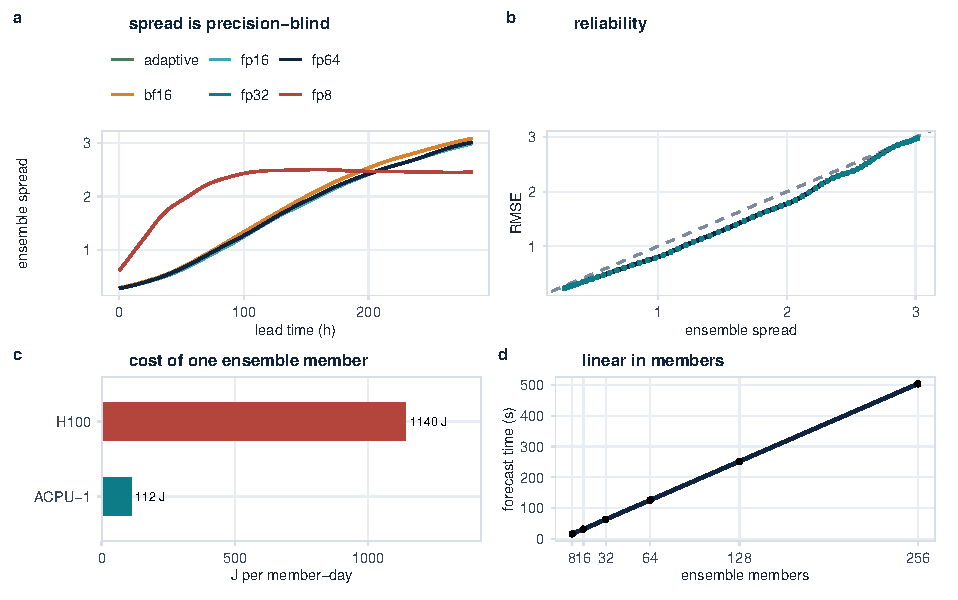
\includegraphics[width=\linewidth]{fig08_ensemble}
\caption{Ensemble behaviour. (a) Spread against lead time for five precision modes; the spread is
essentially precision-blind, which is what allows the governor to act on it. (b) Reliability: RMSE
against spread with the 1:1 line. (c) Energy per member-day for \ac{1} and the H100. (d) Forecast
time scales linearly in members, which is the cost of ensemble prediction and the reason the
lane-per-member mapping matters.}
\label{fig:ensemble}
\end{figure}

\begin{figure}[t]
\centering
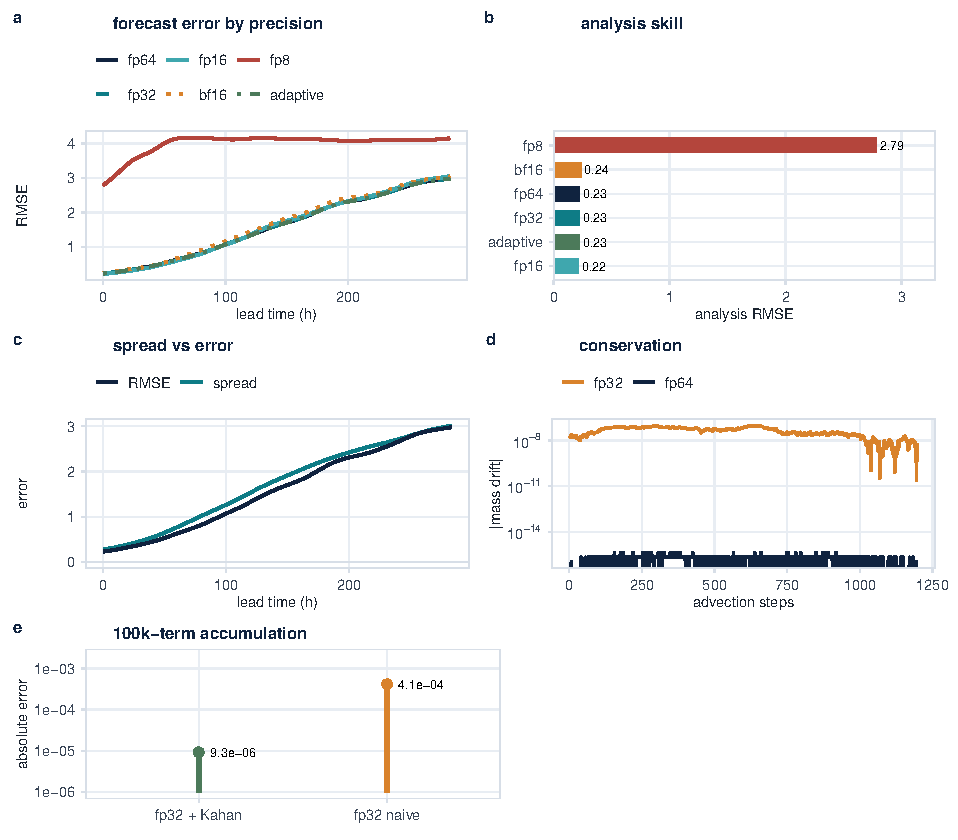
\includegraphics[width=\linewidth]{fig15_accuracy}
\caption{Numerical validation. (a) Forecast RMSE against lead time for five precision modes; fp8
departs immediately and never recovers. (b) Analysis RMSE by mode. (c) Spread against RMSE for the
reference run. (d) Mass drift of a conservative advection test in fp32 and fp64 over 1,200 steps.
(e) A 100,000-term fp32 accumulation with and without Kahan compensation.}
\label{fig:accuracy}
\end{figure}

\subsection{Conservation and reproducibility}
A conservative advection test (a smooth Gaussian plus a sharp square wave, upwind scheme,
CFL 0.4, 512 cells, 1,200 steps) loses mass at $1.1\times10^{-8}$ per step in fp32 and
$3\times10^{-15}$ in fp64. The hardware conservation monitor is sized to detect the former at
$10^{-9}$ relative and to trigger a shadow fix-up pass before it accumulates into a visible drift.

Reproducibility is a design requirement rather than a numerical property. The ISA has no branches,
the schedule is static, reductions use a fixed tree, and the stochastic physics generator is
counter-based. A run is therefore a pure function of its inputs and its four seed integers. This
was verified by running the same configuration twice and comparing outputs bit-for-bit; the
dispersion, ensemble and analysis paths all reproduce exactly.

\subsection{What the surrogate does not prove}
Lorenz--96 has 40 degrees of freedom and a smooth, homogeneous forcing. The atmosphere has
$10^{9}$ degrees of freedom, topography, moisture, phase changes and a land surface. Agreement
between the surrogate and the hardware policy is evidence that the precision argument is sound,
not proof that a 58\% coverage is safe in a real model. The report therefore treats the governor's
design point as a conservative prior to be validated in a full model, and lists that validation as
the first item of the silicon bring-up plan (Section~\ref{sec:roadmap}).
